Cracking tool have to modify the application code since it contains the license verification.
The investigations starts with analysing the \gls{apk}'s \textit{classes.dex}.
The goal is to identify how the circumventing of the license verification mechanism is achieved.
This aquired knowledge is later used to find countermeasures for the crackign tools.
\newline
The reengineering has to be done by using different layers of abstraction.
While dex and smali code reflects local changes, Java code is used to detect functional changes.
It is possible to access the applications Java code since the dex code can be decompiled as seen in figure~\ref{fig:re1}.
This requires different tools which will be explained in this section.
\newline
\begin{figure}[h]
    \centering
    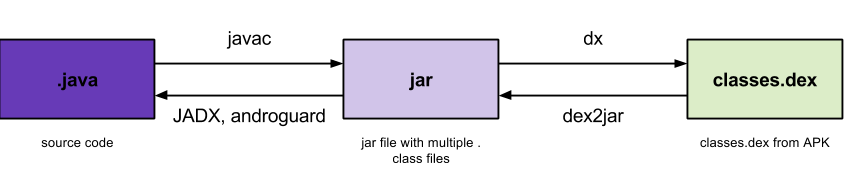
\includegraphics[width=0.8\textwidth]{data/re1.png}
    \caption{Java .class and .dex can be transformed bidirectional \cite{andevconDalvikART}}
    \label{fig:re1}
\end{figure}
